\documentclass{article}

\title{Dummit \& Foote Ch. 2.5: The Lattice of Subgroups of a Group}
\author{Scott Donaldson}
\date{Aug. 2023}
\usepackage{amsmath, amsthm, amsfonts, enumitem, tabu, tikz}

\tikzset{white border/.style={preaction={draw,white,line width=4pt}}}
\newcommand{\gen}[1]{$\langle#1\rangle$} % node text

\begin{document}

\maketitle

\section*{1. (8/11/23)}

Let $H$ and $K$ be subgroups of $G$. Exhibit all possible sublattices which show only $G$, 1, $H$, $K$, and their joins and intersections. What distinguishes the different drawings?

\vspace{0.5cm}

\noindent
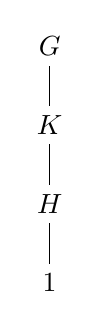
\begin{tikzpicture}
    \node at (0,0)    (I)  {$1$};
    \node at (0,1)    (H) {$H$};
    \node at (0,2)    (K) {$K$};
    \node at (0,3)    (G)  {$G$};
    
    \draw (I) -- (H);
    \draw (H) -- (K);
    \draw (K) -- (G);
\end{tikzpicture}
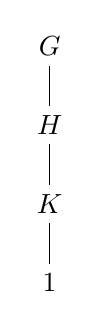
\begin{tikzpicture}
    \node at (0,0)    (I)  {$1$};
    \node at (0,1)    (K) {$K$};
    \node at (0,2)    (H) {$H$};
    \node at (0,3)    (G)  {$G$};
    
    \draw (I) -- (K);
    \draw (K) -- (H);
    \draw (H) -- (G);
\end{tikzpicture}
\begin{tikzpicture}
    \node at (0,0)    (I)  {$1$};
    \node at (1,1.5)    (K) {$K$};
    \node at (-1,1.5)    (H) {$H$};
    \node at (0,3)    (G)  {$G$};
    
    \draw (I) -- (K);
    \draw (I) -- (H);
    \draw (H) -- (G);
    \draw (K) -- (G);
\end{tikzpicture}
\begin{tikzpicture}
    \node at (0,0)    (I)  {$1$};
    \node at (0,1)    (HintK) {$H \cap K$};
    \node at (1,2)   (K) {$K$};
    \node at (-1,2)    (H) {$H$};
    \node at (0,3)    (G)  {$G$};
    
    \draw (I) -- (HintK);
    \draw (HintK) -- (H);
    \draw (HintK) -- (K);
    \draw (H) -- (G);
    \draw (K) -- (G);
\end{tikzpicture}
\begin{tikzpicture}
    \node at (0,0)    (I)  {$1$};
    \node at (1,1)   (K) {$K$};
    \node at (-1,1)    (H) {$H$};
    \node at (0,2)    (HK) {\gen{H,K}};
    \node at (0,3)    (G)  {$G$};
    
    \draw (I) -- (H);
    \draw (I) -- (K);
    \draw (H) -- (HK);
    \draw (K) -- (HK);
    \draw (HK) -- (G);
\end{tikzpicture}
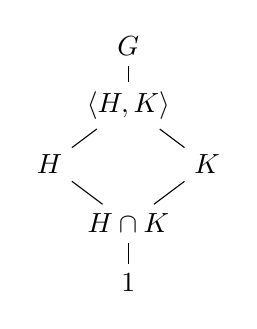
\begin{tikzpicture}
    \node at (0,0)    (I)  {$1$};
    \node at (0,0.75)    (HintK) {$H \cap K$};
    \node at (1,1.5)    (K) {$K$};
    \node at (-1,1.5)   (H) {$H$};
    \node at (0,2.25)    (HK) {\gen{H,K}};
    \node at (0,3)    (G)  {$G$};
    
    \draw (I) -- (HintK);
    \draw (HintK) -- (H);
    \draw (HintK) -- (K);
    \draw (H) -- (HK);
    \draw (K) -- (HK);
    \draw (HK) -- (G);
\end{tikzpicture}

\vspace{0.5cm}

The left two lattices show the group structure when either $H \leq K$ or $K \leq H$ (they omit any subgroups of the smaller of the two, as well as any containing subgroups between the larger and $G$).

The next lattice shows the group structure when $H$ and $K$ are not comparable, their intersection consists only of the identity, and their join is all of $G$. The final three lattices show the cases where $H \cap K$ is a subgroup not equal to the identity, where $\langle H, K \rangle$ is a subgroup not equal to $G$, and where both of these occur.

\section*{2. (8/11/23)}

In each of (a) to (d) list all subgroups of $D_{16}$ that satisfy the given condition.

\begin{enumerate}[label=(\alph*), itemsep=0em]
    \item Subgroups that are contained in $\langle sr^2, r^4 \rangle$

          $\{ 1 \}, \langle sr^6 \rangle, \langle sr^2 \rangle, \langle r^4 \rangle$, $\langle sr^2, r^4 \rangle$
    \item Subgroups that are contained in $\langle sr^7, r^4 \rangle$

        $\{ 1 \}, \langle sr^3 \rangle, \langle sr^7 \rangle, \langle r^4 \rangle$, $\langle sr^7, r^4 \rangle$
    \item Subgroups that contain $\langle r^4 \rangle$

        $\langle r^4 \rangle$, $\langle sr^2, r^4 \rangle, \langle s, r^4 \rangle, \langle r^2 \rangle, \langle sr^3, r^4 \rangle, \langle sr^5, r^4 \rangle, \langle s, r^2 \rangle, \langle r \rangle, \langle sr, r^2 \rangle, D_{16}$
    \item Subgroups that contain $\langle s \rangle$

        $\langle s \rangle$, $\langle s, r^4 \rangle, \langle s, r^2 \rangle, \langle D_{16} \rangle$
\end{enumerate}

\section*{3. (8/11/23)}

Show that the subgroup $\langle s, r^2 \rangle$ of $D_8$ is isomorphic to $V_4$.

\begin{proof}
    The subgroup $\langle s, r^2 \rangle$ of $D_8$ contains the elements $\{ 1, s, r^2, sr^2 \}$. There is no element in this group of order 4. From Ch. 1.1, Exercise 36, there is only one unique group of order 4 with no element of order 4, the Klein group $V_4$. Thus $\langle s, r^2 \rangle$ is isomorphic to $V_4$.
\end{proof}

\section*{4. (8/14/23)}

Use the given lattice to find all pairs of elements that generate $D_8$.

\begin{proof}
    Since $D_8$ is generated by $\langle s, r \rangle$, it suffices to find pairs of elements that generate $s$ and $r$. These pairs of elements are:
    \begin{itemize}[itemsep=0em]
        \item $\langle s, r \rangle$ (trivial)
        \item $\langle s, r^3 \rangle$ ($r = (r^3)^3$)
        \item $\langle s, sr \rangle$ ($r = s \cdot sr$)
        \item $\langle s, sr^3 \rangle$ ($r = s \cdot (sr^3)^3$)
        \item $\langle sr, r \rangle$ ($s = r \cdot sr$)
        \item $\langle sr, r^2 \rangle$ ($r^3 = r^2 \cdot sr, r = (r^3)^3, s = r \cdot sr$)
        \item $\langle sr, r^3 \rangle$ ($r = (r^3)^3, s = r \cdot sr$)
        \item $\langle sr^2, r \rangle$ ($s = sr^2 \cdot r^2$)
        \item $\langle sr^2, r^3 \rangle$ ($r = (r^3)^3, s = sr^2 \cdot r^2$)
        \item $\langle sr^2, sr^3 \rangle$ ($r = sr^2 \cdot sr^3, s = sr^2 \cdot r^2$)
        \item $\langle sr^3, r \rangle$ ($s = sr^3 \cdot r$)
        \item $\langle sr^3, r^3 \rangle$ ($s = r^3 \cdot sr^3, r = s \cdot sr^3$)
    \end{itemize}
\end{proof}

\section*{5. (8/14/23)}

Use the given lattice to find all elements $x \in D_{16}$ such that $D_{16} = \langle x, s \rangle$.

\begin{proof}
    The element $x \in D_{16}$ generates $D_{16}$ together with $s$ if $r$ can be expressed as a product of $s$ and $x$:
    \begin{itemize}[itemsep=0em]
        \item $x = r$ (trivial)
        \item $x = r^3$ ($r = (r^3)^3$)
        \item $x = r^5$ ($r = (r^5)^5$)
        \item $x = r^7$ ($r = (r^7)^7$)
        \item $x = sr$ ($r = s \cdot sr$)
        \item $x = sr^3$ ($r^3 = s \cdot sr^3$, $r = (r^3)^3$)
        \item $x = sr^5$ ($r^5 = s \cdot sr^5$, $r = (r^5)^5$)
        \item $x = sr^7$ ($r^7 = s \cdot sr^7$, $r = (r^7)^7$)
    \end{itemize}
\end{proof}

\section*{6. (8/14/23)}

Find the centralizers of every element in the following groups:

\begin{enumerate}[label=(\alph*), itemsep=0em]
    \item $D_8$
          \begin{itemize}[itemsep=0em]
            \item 1: $D_8$
            \item $r, r^2, r^3$: $\langle r \rangle$
            \item $s, sr^2$: $\langle s, r^2 \rangle$
            \item $sr, sr^3$: $\langle sr, r^2 \rangle$
          \end{itemize}
    \item $Q_8$
          \begin{itemize}[itemsep=0em]
            \item 1, -1: $Q_8$
            \item $i, -i$: $\langle i \rangle$
            \item $j, -j$: $\langle j \rangle$
            \item $k, -k$: $\langle k \rangle$
          \end{itemize}
    \item $S_3$
          \begin{itemize}[itemsep=0em]
            \item $(1)$: $S_3$
            \item $(1, 2)$: $\langle (1, 2) \rangle$
            \item $(1, 3)$: $\langle (1, 3) \rangle$
            \item $(2, 3)$: $\langle (2, 3) \rangle$
            \item $(1, 2, 3), (1, 3, 2)$: $\langle (1, 2, 3) \rangle$
          \end{itemize}
    \item $D_{16}$
          \begin{itemize}[itemsep=0em]
            \item 1: $D_{16}$
            \item $r, r^2, ..., r^7$: $\langle r \rangle$
            \item $s, sr^4$: $\langle s, r^4 \rangle$
            \item $sr, sr^5$: $\langle sr, r^4 \rangle$
            \item $sr^2, sr^6$: $\langle sr^2, r^4 \rangle$
            \item $sr^3, sr^7$: $\langle sr^3, r^4 \rangle$
          \end{itemize}
\end{enumerate}

\section*{7. (8/14/23)}

Find the center of $D_{16}$.

\begin{proof}
    From the preceding exercise, the only elements that are in the centralizer of every element of $D_{16}$ are $\{ 1, r^4 \} = \langle r^4 \rangle$.
\end{proof}

\section*{8. (8/14/23)}

In each of the following groups find the normalizer of each subgroup:

\begin{enumerate}[label=(\alph*), itemsep=0em]
    \item $S_3$: The subgroups (other than $(1)$ and all of $S_3$) are the three cyclic groups generated by the each of the 2-cycles, and the group consisting of $\{ (1), (1, 2, 3), (1, 3, 2) \}$. In the case of $\langle (1, 2) \rangle$, notice that:
    \begin{equation*}
        (1, 3)(1, 2)(1, 3)^{-1} = (1, 3)(1, 2)(1, 3) = (2, 3) \notin \langle (1, 2) \rangle,
    \end{equation*}
    which implies that $(1, 3) \notin N_{S_3}((1, 2))$. By extension, no 2-cycle is in the normalizer of another 2-cycle. There is no subgroup of $S_3$ that contains a 2-cycle, a 3-cycle, but does \emph{not} contain a different 2-cycle. Therefore each cyclic subgroup of $S_3$ is its own normalizer.

    Now for the subgroup $\{ (1), (1, 2, 3), (1, 3, 2) \}$, we have $(1, 2)(1, 2, 3)(1, 2) = (1, 3, 2)$, which is included in the subgroup. It follows that the normalizer of this subgroup is all of $S_3$.
    \item $Q_8$: The elements 1 and $-1$ commute with all elements of $Q_8$, so the normalizer of $\langle -1 \rangle$ is all of $Q_8$. Consider the normalizer of $\langle i \rangle$. Now $j \cdot i \cdot j^{-1} = j \cdot i \cdot -j = -k \cdot -j = i$, so $j \in N_{Q_8}(\langle i \rangle)$. Then the normalizer of $i$ contains at least 5 elements, so it must be all of $Q_8$. By extension, every subgroup of $Q_8$ is its own normalizer.
\end{enumerate}

\section*{9. (8/14/23)}

Draw the lattices of subgroups of the following groups:

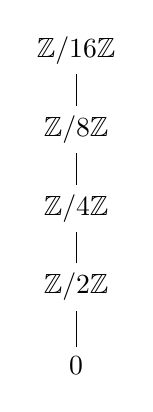
\begin{tikzpicture}
    \node at (0,0)    (1)  {$0$};
    \node at (0,1)    (2)  {$\mathbb{Z}/2\mathbb{Z}$};
    \node at (0,2)    (4)  {$\mathbb{Z}/4\mathbb{Z}$};
    \node at (0,3)    (8)  {$\mathbb{Z}/8\mathbb{Z}$};
    \node at (0,4)    (16) {$\mathbb{Z}/16\mathbb{Z}$};
    
    \draw (1) -- (2);
    \draw (2) -- (4);
    \draw (4) -- (8);
    \draw (8) -- (16);
\end{tikzpicture}\hspace{1cm}
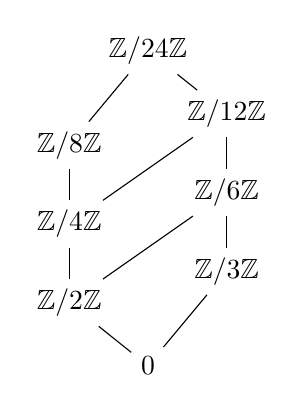
\begin{tikzpicture}
    \node at (0,0)          (1)  {$0$};
    \node at (-1,0.8)      (2)  {$\mathbb{Z}/2\mathbb{Z}$};
    \node at (1,1.2)       (3)  {$\mathbb{Z}/3\mathbb{Z}$};
    \node at (-1,1.8)      (4)  {$\mathbb{Z}/4\mathbb{Z}$};
    \node at (1,2.2)       (6)  {$\mathbb{Z}/6\mathbb{Z}$};
    \node at (-1,2.8)      (8)  {$\mathbb{Z}/8\mathbb{Z}$};
    \node at (1,3.2)       (12) {$\mathbb{Z}/12\mathbb{Z}$};
    \node at (0,4)          (24) {$\mathbb{Z}/24\mathbb{Z}$};
    
    \draw (1) -- (2);
    \draw (1) -- (3);
    \draw (2) -- (4);
    \draw (2) -- (6);
    \draw (4) -- (8);
    \draw (4) -- (12);
    \draw (8) -- (24);
    \draw (3) -- (6);
    \draw (6) -- (12);
    \draw (12) -- (24);
\end{tikzpicture}\hspace{1cm}
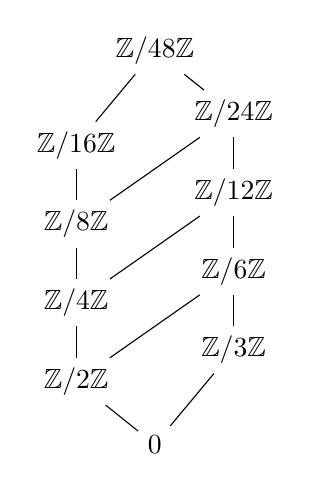
\begin{tikzpicture}
    \node at (0,0)          (1)  {$0$};
    \node at (-1,0.8)      (2)  {$\mathbb{Z}/2\mathbb{Z}$};
    \node at (1,1.2)       (3)  {$\mathbb{Z}/3\mathbb{Z}$};
    \node at (-1,1.8)      (4)  {$\mathbb{Z}/4\mathbb{Z}$};
    \node at (1,2.2)       (6)  {$\mathbb{Z}/6\mathbb{Z}$};
    \node at (-1,2.8)      (8)  {$\mathbb{Z}/8\mathbb{Z}$};
    \node at (1,3.2)       (12) {$\mathbb{Z}/12\mathbb{Z}$};
    \node at (-1,3.8)      (16)  {$\mathbb{Z}/16\mathbb{Z}$};
    \node at (1,4.2)          (24) {$\mathbb{Z}/24\mathbb{Z}$};
    \node at (0,5)          (48) {$\mathbb{Z}/48\mathbb{Z}$};
    
    \draw (1) -- (2);
    \draw (1) -- (3);
    \draw (2) -- (4);
    \draw (2) -- (6);
    \draw (4) -- (8);
    \draw (4) -- (12);
    \draw (8) -- (24);
    \draw (8) -- (16);
    \draw (3) -- (6);
    \draw (6) -- (12);
    \draw (12) -- (24);
    \draw (16) -- (48);
    \draw (24) -- (48);
\end{tikzpicture}

\section*{10. (8/15/23)}

Classify groups of order 4 by proving that if $|G| = 4$ then $G \cong Z_4$ or $G \cong V_4$.

\begin{proof}
    From Ch. 1.1, Exercise 36, if $G$ is a group with 4 elements and no element of order 4, then we must have $G = \langle a, b \mid a^2 = b^2 = 1, ab = ba \rangle \cong V_4$.

    If $G$ does have an element of order 4, then we have the cyclic group $G = \langle a \mid a^4 = 1 \rangle \cong Z_4$. All cyclic groups of equal order are isomorphic.

    Therefore a group of order 4 must be isomorphic to either the cyclic group of order 4 or the Klein 4-group.
\end{proof}

\section*{11. (8/15/23)}

Consider the group of order 16 with the following presentation:

\begin{equation*}
    QD_{16} = \langle \sigma, \tau \mid \sigma^8 = \tau^2 = 1, \sigma \tau = \tau \sigma^3 \rangle
\end{equation*}

(called the \emph{quasidihedral} or \emph{semidihedral} group of order 16). This group has three subgroups of order 8: $\langle \tau, \sigma^2 \rangle \cong D_8, \langle \sigma \rangle \cong Z_8$ and $\langle \sigma^2, \sigma \tau \rangle \cong Q_8$ and every proper subgroup is contained in one of these three subgroups. Fill in the lattice of all subgroups of the quasidihedral group, exhibiting each subgroup with at most two generators.

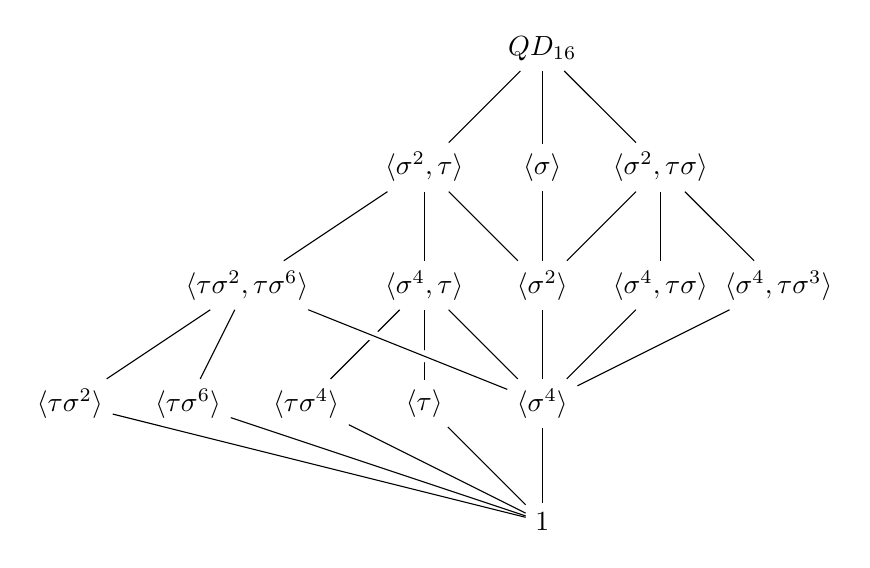
\begin{tikzpicture}[x=1.5cm,y=1.5cm]
    \node at (0,0)          (1)  {$1$};
    \node at (0, 1)      (s4)  {$\langle \sigma^4 \rangle$};
    \node at (-1, 1)      (t)  {$\langle \tau \rangle$};
    \node at (-2, 1)      (ts4)  {$\langle \tau \sigma^4 \rangle$};
    \node at (-3, 1)      (ts6)  {$\langle \tau \sigma^6 \rangle$};
    \node at (-4, 1)      (ts2)  {$\langle \tau \sigma^2 \rangle$};
    \node at (-1, 2)       (s4-t)  {$\langle \sigma^4, \tau \rangle$};
    \node at (-2.5, 2)       (ts2-ts6)  {$\langle \tau \sigma^2, \tau \sigma^6 \rangle$};
    \node at (0, 2)       (s2)  {$\langle \sigma^2 \rangle$};
    \node at (1, 2)       (s4-ts)  {$\langle \sigma^4, \tau \sigma \rangle$};
    \node at (2, 2)       (s4-ts3)  {$\langle \sigma^4, \tau \sigma^3 \rangle$};
    \node at (-1, 3)      (s2-t)  {$\langle \sigma^2, \tau \rangle$};
    \node at (0, 3)      (s)  {$\langle \sigma \rangle$};
    \node at (1, 3)      (s2-ts)  {$\langle \sigma^2, \tau \sigma \rangle$};
    \node at (0, 4)       (QD16)  {$QD_{16}$};
    
    \draw (1) -- (s4);
    \draw (1) -- (t);
    \draw (1) -- (ts4);
    \draw (1) -- (ts6);
    \draw (1) -- (ts2);
    \draw (s4) -- (s4-t);
    \draw (t) -- (s4-t);
    \draw (ts4) -- (s4-t);
    \draw (s4) -- (ts2-ts6);
    \draw (ts2) -- (ts2-ts6);
    \draw (ts6) -- (ts2-ts6);
    \draw (s4) -- (s2);
    \draw (s4) -- (s4-ts);
    \draw (s4) -- (s4-ts3);
    \draw (ts2-ts6) -- (s2-t);
    \draw (s4-t) -- (s2-t);
    \draw (s2) -- (s2-t);
    \draw (s2) -- (s);
    \draw (s2) -- (s2-ts);
    \draw (s4-ts) -- (s2-ts);
    \draw (s4-ts3) -- (s2-ts);
    \draw (s) -- (QD16);
    \draw (s2-ts) -- (QD16);
    \draw (s2-t) -- (QD16);

    \draw[white border] (s4) -- (ts2-ts6);
\end{tikzpicture}

\section*{12. (8/16/23)}

The group $A = Z_2 \times Z_4 = \langle a, b \mid a^2 = b^4 = 1, ab = ba \rangle$ has order 8 and has three subgroups of order 4: $\langle a, b^2 \rangle \cong V_4, \langle b \rangle \cong Z_4$ and $\langle ab \rangle \cong Z_4$ and every proper subgroup is contained in one of these three. Draw the lattice of all subgroups of $A$, giving each subgroup in terms of at most two generators.

\begin{center}
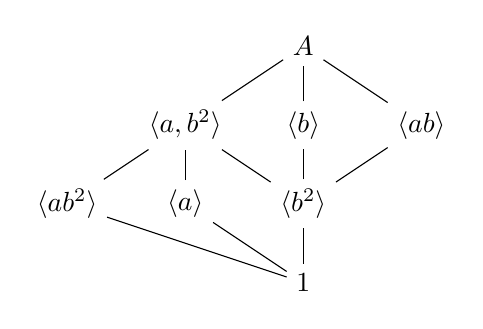
\begin{tikzpicture}[x=1.5cm]
    \node at (0,0)          (1)  {$1$};
    \node at (0, 1)      (b2)  {$\langle b^2 \rangle$};
    \node at (-1, 1)      (a)  {$\langle a \rangle$};
    \node at (-2, 1)      (ab2)  {$\langle ab^2 \rangle$};
    \node at (-1, 2)      (a-b2)  {$\langle a, b^2 \rangle$};
    \node at (0, 2)       (b)  {$\langle b \rangle$};
    \node at (1, 2)       (ab)  {$\langle ab \rangle$};
    \node at (0, 3)       (A)  {$A$};
    
    \draw (1) -- (b2);
    \draw (1) -- (ab2);
    \draw (1) -- (a);
    \draw (b2) -- (b);
    \draw (b2) -- (ab);
    \draw (b2) -- (a-b2);
    \draw (ab2) -- (a-b2);
    \draw (a) -- (a-b2);
    \draw (a-b2) -- (A);
    \draw (b) -- (A);
    \draw (ab) -- (A);
\end{tikzpicture}
\end{center}

\section*{13. (8/16/23)}

The group $G = Z_2 \times Z_8 = \langle x, y \mid x^2 = y^8 = 1, xy = yx \rangle$ has order 16 and has three proper subgroups of order 8: $\langle x, y^2 \rangle \cong Z_2 \times Z_4, \langle y \rangle \cong Z_8$ and $\langle xy \rangle \cong Z_8$ and every proper subgroup is contained in one of these three. Draw the lattice of all subgroups of $G$, giving each subgroup in terms of at most two generators.

\begin{center}
    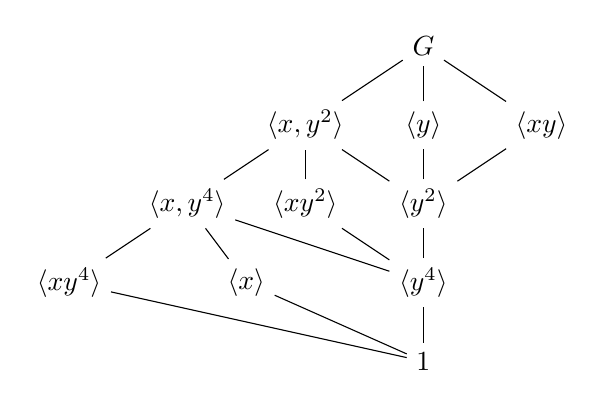
\begin{tikzpicture}[x=1.5cm]
        \node at (0,0)          (1)  {$1$};
        \node at (0, 1)      (y4)  {$\langle y^4 \rangle$};
        \node at (-1.5, 1)      (x)  {$\langle x \rangle$};
        \node at (-3, 1)      (xy4)  {$\langle xy^4 \rangle$};
        \node at (-2, 2)      (x-y4)  {$\langle x, y^4 \rangle$};
        \node at (-1, 2)      (xy2)  {$\langle xy^2 \rangle$};
        \node at (0, 2)      (y2)  {$\langle y^2 \rangle$};
        \node at (-1, 3)      (x-y2)  {$\langle x, y^2 \rangle$};
        \node at (0, 3)      (y)  {$\langle y \rangle$};
        \node at (1, 3)      (xy)  {$\langle xy \rangle$};
        \node at (0, 4)      (G)  {$G$};
        
        \draw (1) -- (y4);
        \draw (1) -- (x);
        \draw (1) -- (xy4);
        \draw (y4) -- (x-y4);
        \draw (x) -- (x-y4);
        \draw (xy4) -- (x-y4);
        \draw (y4) -- (xy2);
        \draw (y4) -- (y2);
        \draw (x-y4) -- (x-y2);
        \draw (xy2) -- (x-y2);
        \draw (y2) -- (x-y2);
        \draw (y2) -- (y);
        \draw (y2) -- (xy);
        \draw (x-y2) -- (G);
        \draw (y) -- (G);
        \draw (xy) -- (G);
    \end{tikzpicture}
\end{center}

\section*{14. (8/17/23)}

Let $M$ be the group of order 16 with the following presentation:
\begin{equation*}
    \langle u, v \mid u^2 = v^8 = 1, vu = uv^5 \rangle
\end{equation*}
(sometimes called the \emph{modular} group of order 16). It has three subgroups of order 8: $\langle u, v^2 \rangle, \langle v \rangle$ and $\langle uv \rangle$ and every proper subgroup is contained in one of these three. Prove that $\langle u, v^2 \rangle \cong Z_2 \times Z_4$, $\langle v \rangle \cong Z_8$ and $\langle uv \rangle \cong Z_8$. Show that the lattice of subgroups of $M$ is the same as the lattice of subgroups of $Z_2 \times Z_8$ but that these two groups are not isomorphic.

\begin{proof}
    Given that the generator $v$ has order 8, the cyclic subgroup generated by $v$ must be isomorphic to $Z_8$.

    Consider next $\langle u, v^2 \rangle = \{ 1, v^2, v^4, v^6, uv^2, uv^4, uv^6 \}$. Does this cyclic subgroup contain any more elements? We have $v^2 u = u(v^2)^5 = uv^{10} = uv^2$, so $u$ and $v^2$ commute. Therefore higher powers of $v^2$ also commute with $u$, so there are no more elements in this generated subgroup. Define a map $\varphi: \langle u, v^2 \rangle \rightarrow Z_2 \times Z_4$ by $\varphi(u) = (1, 0)$ and $\varphi(v^2) = (0, 1)$. The group $Z_2 \times Z_4$ is generated by $(1, 0)$ and $(0, 1)$, so $\varphi$ is surjective, and since the two groups have the same order, $\varphi$ is an isomorphism. It follows that $\langle u, v^2 \rangle \cong Z_2 \times Z_4$.

    Further consider $\langle uv \rangle$. We have $(uv)^8 = ((uv)^2)^4 = (uvuv)^4 = (uuv^5 v)^4 = (v^6)^4 = v^{24} = 1$. So the order of $uv$ must divide 8. From above, we know that $(uv)^2 = v^6 \neq 1$. And $(uv)^4 = ((uv)^2)^2 = (v^6)^2 = v^{12} = v^4 \neq 1$. Therefore $|uv| = 8$, so $\langle uv \rangle \cong Z_8$.

    The three maximal subgroups of $M$ are isomorphic to the three maximal subgroups of $Z_2 \times Z_8$ (Exercise 13). However, $M$ is not abelian and $Z_2 \times Z_8$ is abelian. Might they still be isomorphic? Let $x, y \in M$ with $xy \neq yx$. Suppose that $\varphi: M \rightarrow Z_2 \times Z_8$ is an isomorphism and that $\varphi(x) = g, \varphi(y) = h \in Z_2 \times Z_8$. So we have $gh = \varphi(x) \varphi(y) = \varphi(xy)$ and $hg = \varphi(y) \varphi(x) = \varphi(yx)$. However, we have $gh = hg$ (because $Z_2 \times Z_8$ is abelian), and $xy \neq yx \Rightarrow \varphi(xy) \neq \varphi(yx)$, a contradiction. Therefore no abelian group is isomorphic to a non-abelian group.
\end{proof}

\section*{15. (8/17/23)}

Describe the isomorphism type of each of the three subgroups of $D_{16}$ of order 8.

\begin{proof}
    Given the lattice of subgroups of $D_{16}$, there are three subgroups of order 8: $\langle r \rangle, \langle sr \rangle$, and $\langle s, r^2 \rangle$. Since the first two are generated by single elements, they are both isomorphic to the cyclic group $Z_8$.

    So consider $\langle s, r^2 \rangle = \{ 1, r^2, r^4, r^6, s, sr^2, sr^4, sr^6 \}$. Let $\varphi: \langle s, r^2 \rangle \rightarrow D_8$ be defined by $\varphi(s) = s_4$ and $\varphi(r^2) = r_4$ (where the subscripts denote those elements in $D_8$ as opposed to $D_{16}$). Now $\varphi$ is a map defined on the generators of $\langle s, r^2 \rangle$ to the generators of $D_8$, and since the two groups have the same order, it is an isomorphism and therefore $\langle s, r^2 \rangle \cong D_8$.
\end{proof}

\section*{16. (8/18/23)}

Use the lattice of subgroups of the quasidihedral group of order 16 to show that every element of order 2 is contained in the proper subgroup $\langle \tau, \sigma^2 \rangle$.

\begin{proof}
    In $QD_{16}$, there are 5 elements of order 2: $\sigma^4, \tau, \tau \sigma^2, \tau \sigma^4$, and $\tau \sigma^6$. We start by considering the cyclic subgroup generated by each and note that $\langle \sigma^4 \rangle, \langle \tau \rangle, \langle \tau \sigma^4 \rangle \leq \langle \tau, \sigma^4 \rangle$ and that $\langle \tau \sigma^2 \rangle, \langle \tau \sigma^6 \rangle \leq \langle \tau \sigma^2, \tau \sigma^6 \rangle$. We find the join of these two subgroups in $\langle \tau, \sigma^2 \rangle$ and so every element of order 2 is contained in this subgroup.
\end{proof}

\section*{17. (8/18/23)}

Use the lattice of subgroups of the modular group $M$ of order 16 to show that the set $\{ x \in M \mid x^2 = 1 \}$ is a subgroup of $M$ isomorphic to the Klein 4-group.

\begin{proof}
    The subset $\{ x \in M \mid x^2 = 1 \}$ consists of every element of order 2 together with the identity, that is, $\{ 1, u, v^4, uv^4 \}$. Since this is a set of 4 elements with an identity that is closed and closed under inverses (since each element is its own inverse), it is a subgroup and therefore a group. There is no element with order 4, so it must be isomorphic to the Klein 4-group.
\end{proof}

\section*{18. (8/18/23)}

Find the centralizer of every element of $QD_{16}$.

\begin{itemize}[itemsep=0em]
    \item $Z(1) = QD_{16}$ (trivial)
    \item $Z(\sigma) = Z(\sigma^2) = Z(\sigma^3) = Z(\sigma^5) = Z(\sigma^6) = Z(\sigma^7) = \langle \sigma \rangle$: $\tau$ does not commute with these elements and so cannot be an element of their centralizer, however, all powers of $\sigma$ commute with each other
    \item $Z(\sigma^4) = QD_{16}$: $\tau$ \emph{does} commute with $\sigma^4$, and since $\sigma^4 \in \langle \sigma \rangle$, we have $Z(\sigma^4) = \langle \tau, \sigma \rangle = QD_{16}$
    \item $Z(\tau) = Z(\tau \sigma^4) = \langle \tau, \sigma^4 \rangle$: Of the powers of $\sigma$, only $\sigma^4$ commutes with $\tau$, and the other elements $\tau \sigma^k$ do not commute with $\tau$
    \item $Z(\tau \sigma) = Z(\tau \sigma^5) = \langle \sigma^4, \tau \sigma \rangle$
    \item $Z(\tau \sigma^2) = Z(\tau \sigma^6) = \langle \tau \sigma^2, \tau \sigma^6 \rangle$
    \item $Z(\tau \sigma^3) = Z(\tau \sigma^7) = \langle \sigma^4, \tau \sigma^3 \rangle$
\end{itemize}

\section*{19. (8/19/23)}

Find $N_{D_{16}}(\langle s, r^4 \rangle)$.

\begin{proof}
    An element always belongs to its normalizer, so in considering candidates for the normalizer of $\langle s, r^4 \rangle$ in $D_{16}$, we only have to consider subgroups containing $\langle s, r^4 \rangle$. There are only two possibilities, the generated subgroup $\langle s, r^2 \rangle$ and the entire group $D_{16}$ itself.

    We note that the conjugate of $s$ by $r^2$ is $r^2 s r^6 = s r^6 r^6 = sr^{12} = sr^4$, which lies in $\langle s, r^4 \rangle$. Since $r^2$ commutes with $r^4$, we must have $r^2 \in N_{D_{16}}(\langle s, r^4 \rangle)$. Therefore $\langle s, r^2 \rangle \leq N_{D_{16}}(\langle s, r^4 \rangle)$.

    Next, note that the conjugate of $s$ by $r$ is $r s r^7 = sr^7 r^7 = sr^{14} = sr^6 \notin \langle s, r^4 \rangle$. Therefore $r$ is not in the normalizer of $\langle s, r^4 \rangle$, and so the entire group $D_{16}$ is not a candidate. Thus we must have $N_{D_{16}}(\langle s, r^4 \rangle) = \langle s, r^2 \rangle$.
\end{proof}

\section*{20. (8/19/23)}

Find the following normalizers in $QD_{16}$:

\begin{enumerate}[label=(\alph*), itemsep=0em]
    \item $N_{QD_{16}}(\langle \tau \sigma \rangle)$
    
        We only have to check subgroups containing $\langle \tau \sigma \rangle$, namely $\langle \sigma^2, \tau \sigma \rangle$ and the entire group $QD_{16}$. In $\langle \sigma^2, \tau \sigma \rangle$, $\tau \sigma$ is in its own normalizer, so consider the conjugate:
        \begin{equation*}
            \sigma^2 \tau \sigma \sigma^6 = \tau \sigma^6 \sigma \sigma^6 = \tau \sigma^{13} = \tau \sigma^5.
        \end{equation*}
        Since $\tau \sigma^5 \in \langle \tau \sigma \rangle$, we have $\sigma^2 \in N_{QD_{16}}(\langle \tau \sigma \rangle)$, so $\langle \sigma^2, \tau \sigma \rangle \leq N_{QD_{16}}(\langle \tau \sigma \rangle)$.

        Next we consider an element of $QD_{16}$ not in $\langle \sigma^2, \tau \sigma \rangle$, namely $\tau$. The conjugate $\tau \tau \sigma \tau = \sigma \tau = \tau \sigma^3$ is not in the given subgroup $\langle \tau \sigma \rangle$, so $\tau$ is not in the normalizer. Thus $N_{QD_{16}}(\langle \tau \sigma \rangle) = \langle \sigma^2, \tau \sigma \rangle$.
    \item $N_{QD_{16}}(\langle \tau, \sigma^4 \rangle)$
        
        Again, we consider subgroups containing $\langle \tau, \sigma^4 \rangle$; these are $\langle \sigma^2, \tau \rangle$ and the entire group $QD_{16}$. Now $\sigma^2 \tau \sigma^6 = \tau \sigma^6 \sigma^6 = \tau \sigma^{12} = \tau \sigma^4$, which is in the subgroup $\langle \tau, \sigma^4 \rangle$. So $\langle \sigma^2, \tau \rangle \leq N_{QD_{16}}(\langle \tau, \sigma^4 \rangle)$. However, $(\tau \sigma)\tau(\tau \sigma) = \tau \sigma^2 \notin \langle \tau, \sigma^4 \rangle$, so the entire group $QD_{16}$ is not the normalizer. Thus $N_{QD_{16}}(\langle \tau, \sigma^4 \rangle) = \langle \sigma^2, \tau \rangle$.
\end{enumerate}

\end{document}